\documentclass{beamer}
\usepackage[german]{babel}
%\usepackage{libertine}
%\renewcommand*\familydefault{\sfdefault}  %%
\usepackage[default]{opensans}
%\usepackage{gillius2}
%\usepackage{lato}
\usepackage{siunitx}

\usepackage[utf8]{inputenc}

\usepackage[T1]{fontenc}

\usepackage{booktabs} % To thicken table lines
\usepackage{multirow}


\usepackage{microtype}
\usepackage{xcolor,multido,colortbl}
\usepackage{pgffor}

\usepackage{tikz}
\usepackage[version=4]{mhchem}
\usepackage{tikzorbital}

\usepackage{pgfplots}
\pgfplotsset{compat=1.13} 
 %\pgfplotsset{com  =1.13}
\usepackage{graphicx}
\usepackage{adjustbox}
\usepackage{hyperref}
\usepackage{caption}

\usepgfmodule{matrix} 
\usetikzlibrary{matrix,positioning}
\usetikzlibrary{arrows}
\usetikzlibrary{calc,shapes}
\usetikzlibrary{backgrounds}
\newcommand{\makemycolor}[2]{%
    \pgfmathsetmacro{\hue}{(#1/100)^1.715*0.79}%
    \definecolor{myhsbcolor}{hsb}{\hue,1,1}%
    \textcolor{myhsbcolor}{#2}%
}

\usepackage[absolute,overlay]{textpos}




\tikzset{
    level1/.style = {
        ultra thick,
        green
    },
    level4/.style = {
        ultra thick,
        blue
    },
    level5/.style = {
        ultra thick,
        red
    }
}

\newcommand\ytl[2]{
\parbox[b]{8em}{\hfill{\color{cyan}\bfseries\sffamily #1}~$\cdots\cdots$~}\makebox[0pt][c]{$\bullet$}\vrule\quad \parbox[c]{4.5cm}{\vspace{7pt}\color{red!40!black!80}\raggedright\sffamily #2.\\[7pt]}\\[-3pt]}
%\usepackage[texcoord,grid,gridunit=mm,gridcolor=red!10,subgridcolor=green!10]{eso-pic}
\setbeamertemplate{navigation symbols}{}


\title{Lumineszenz von Seltenerd-Ionen}
\author{Nevroz Arslan}

\begin{document}
  {%
    \setbeamertemplate{headline}{}
   \setbeamercolor{postit}{fg=black,bg=yellow}
    \frame{\titlepage}
  }

\begin{frame}[t]\frametitle{Was macht einen guten Leuchtstoff aus?}
\pause
\begin{itemize}
   \item hohe Quantenausbeute $QE = \frac{\text{emittierte \ Photonen}}{\text{absorbierte Photonen}}\%$
   \pause
   \item hohe Übergangswahrscheinlichkeit, kurze Lebensdauer und scharfe Emission 
   \pause
   \item geringe Neigung zu strahlungsloser Relaxation \ce{Ln^* -> Ln +} Wärme
\end{itemize}
   
\end{frame}

\begin{frame}[t]\frametitle{Was macht ein Leuchtstoff bunt?}

\begin{columns}
   \column{.7\textwidth}
    \begin{itemize}
    \item \footnotesize Farbe besteht aus Strahlung unterschiedlicher Wellenlänge
    \item \footnotesize {\color[RGB]{255,0,0}Rot} hat nur Rot (R: 255 G:0 B:0)
        \item \footnotesize {\color[RGB]{255,255,0}Gelb} enthält kein Blau (R: 255 G:255 B:0)
    \item \footnotesize {\color[RGB]{255,0,255}Magenta} enthält kein Grün (R: 255 G:0 B:255)
    \item \footnotesize {\color[RGB]{255, 192, 203} Rosa }hat  R: 255, G:192, B:203 
  % \item Lila ist dunkles Purpur.
    \end{itemize}
   \column{.3\textwidth}
      \begin{tikzpicture}
    \foreach \k in {0,1,...,100}{%
        \pgfmathsetmacro{\hue}{(\k/100)^1.715*0.79}
        \definecolor{mycolor}{rgb:hsb}{\hue,1,1}
        \node[color=mycolor] () at (0,\k/20) {$\bullet$};
    }%
    \foreach \f in {0,1,...,10}{%
        \pgfmathtruncatemacro{\num}{(\f*40)+380}
        \node () at (0.75,\f/2) {$\num$ nm};
    }
    \foreach \g/\h in {0/Rot,2/Orange,4/Gelb,6/Grün,8/Blau,10/Purpur}{%
        \pgfmathtruncatemacro{\num}{\g*10}
        \node at (-1,\g/2) {\makemycolor{\num}{\h}};
    }%
    \end{tikzpicture}

\end{columns}

\end{frame}

%Ein Farbraum beschreibt die Menge der darstellbaren Farben eines Mediums 

\begin{frame}[t]\frametitle{Die drei natürlichen Komponenten der Farbe}
  
\begin{itemize}
      \item Farbton, (Wellenlänge,\textbf{hue}) %\multido{\nColr=0+1}{10}{\fcolorbox{white}{H!![\nColr]}{}}
      \begin{tikzpicture}
          \colorlet{color min hsb}[hsb]{red}
  \colorlet{color max hsb}[hsb]{violet}
   \foreach \pos in {100,...,0}{
    \colorlet{my color hsb}[rgb]{color min hsb!\pos!color max hsb}
    \fill[fill=my color hsb,draw=none] (-3+\pos/20,0) rectangle +(5mm,3mm);
  }
      \end{tikzpicture}
   \item Sättigung (Weißanteil?) 
   \begin{itemize}
   \item Gesättigte Farben -> die spektrale Reinheit 
   \item Ungesättigte Farben sind unbunte Farben (schwarz, grau, weiß).
   \item Farben mit geringer Sättigung werden Pastellfarben genannt
   \end{itemize}
\begin{tikzpicture}
          \colorlet{color min hsb}[hsb]{white}
  \colorlet{color max hsb}[hsb]{red}
   \foreach \pos in {100,...,0}{
    \colorlet{my color hsb}[rgb]{color max hsb!\pos!}
    \fill[fill=my color hsb,draw=none] (-3+\pos/20,0) rectangle +(5mm,3mm);
  }
      \end{tikzpicture}


      \item Helligkeit (Intensität ) %\multido{\nColr=0+1}{10}{\fcolorbox{white}{B!![\nColr]}{}}
      \begin{itemize}
        \item  wird am Model eines Schwarzkörpers analysiert
      \end{itemize}
      
   \end{itemize}


 \end{frame}


\begin{frame}[t]\frametitle{Helligkeit am Model eines Schwarzkörpers }
     \begin{itemize}
     \item \footnotesize Die gesamte ausgestrahlte Energie $P$ in \si{\watt}
     \item \footnotesize nach Boltzmann 
     \item $P = \epsilon(T) \cdot \sigma \cdot A \cdot T^4$
     \begin{itemize}
        \item \footnotesize einer Oberflächen $A$
       \item \footnotesize  proportional zur vierten Potenz der Temperatur
      \item  \footnotesize $\epsilon(T)$ ist materialabhängig
      \end{itemize}    
     \end{itemize}
     \pause
   \begin{table}[!h]
\centering
      \begin{tabular}{ccc}
\toprule
\multirow{2}{*}{Material}&   Temperatur &  Emissivität  \\
& $T$ \si{\celsius}& $\epsilon(T)$\\
\midrule
 Wasser  & 10...50 &0,965  \\
 Sand & 20& 0,76\\
 Eisen,poliert & -73...727 & 0,32...0,60 \\
 Alufolie & 298 & 0.03 \\
\bottomrule
\end{tabular}
\caption{Beispiele für Emissionsgrade einiger Oberflächen}
\end{table}


\end{frame}


%Mit zunehmender Temperatur verschiebt sich die maximale Strahlungsintensität eines Schwarzen Körpers zu kürzeren Wellenlängen, der Farbeindruck wechselt dabei vom Roten ins Bläulich-Weiße. Der Farbton einer (Wärme-) Lichtquelle lässt sich als Temperatur eines vergleichbaren Schwarzen Strahlers angeben. Damit erhält man die Farbtemperatur der Lichtquelle.
\begin{frame}[t]\frametitle{Farbtemperatur}
\begin{itemize}
  \item Plancksverteilungs
  \begin{itemize}
  \item \small Bei niedrigen Temperaturen wird hauptsächlich rotes Licht
  \item \small bei hohen Temperaturen blaues Licht abgestrahlt.
\end{itemize}
\pause
\end{itemize}

\begin{figure}[!h]
\centering
      
\includegraphics[width=\textwidth]{pics/ct.png}
      \caption*{\footnotesize Farbtemperatur nach dem Planckschen Strahlungsgesetz}
 \end{figure}

\end{frame}

   \begin{frame}[t]\frametitle{Farbtemperatur}
       
   

\begin{table}[!h]
\centering
\resizebox{5cm}{!}{
      \begin{tabular}{cc}
\toprule
Lichtquelle &Farbtemperatur \si{\kelvin}\\
\midrule
Blauer Himmel & 10000\\ 
Schattig  &7500 \\
Bewölkter Himmel & 6500 \\
Gebirge &6500 \\
Tageslicht & 5600 \\
Elektronenblitz & 5500 \\
 Abendsonne & 5000 \\
Halogenleuchte & 3400 \\
Glühlampe &2600 \\
Kerze &1500 \\
\bottomrule\\
\end{tabular}
}

\caption*{Beispiele für Farbtemperaturen}
\end{table}

   
   \end{frame}

% \begin{frame}[t]\frametitle{Wiensches Verschiebungsgesetz: }
% Die einfachste Verknüpfung der Strahlungsintensität mit der Wellenlänge     
% \begin{equation}
%     \lambda _{max}=\frac{2897,7 \mu m \cdot K}{T}
%   \end{equation}
%   \begin{itemize}
%   \item \footnotesize $\lambda _{max}$ Wellenlänge $\mu m$, bei der die Intensität pro Wellenlängenintervall maximal ist
%   \item \footnotesize  $T$: absolute Temperatur der strahlenden Fläche
% \end{itemize}
% \end{frame}



%Je höher die Temperatur eines Körpers ist, bei desto kürzeren Wellenlängen liegt das Maximum der Verteilung. 
%Die Wellenlänge maximaler Strahlungsleistung verschiebt sich also bei einer Temperaturänderung einfach umgekehrt proportional zur absoluten Temperatur des schwarzen Strahlers: Verdoppelt sich die Temperatur des Strahlers, so tritt die größte Strahlungsleistung bei der halben Wellenlänge auf.

 %Glasperlen mit Oxiden der Lanthaniden

\begin{frame}[t]\frametitle{Schalenaufbau}
    
   
    \begin{adjustbox}{max totalsize={.9\textwidth}{\textheight},center}
\begin{tikzpicture}
\draw [->,ultra thick] (0,0) --   (0,10) node[above] {\Large Energie};
\draw [->,ultra thick] (0,0) -- node[below] {\Large n (Schale)} (20,0);
    \draw[level4] (6,1) -- node[above] {4s} (7,1);
       \draw[level4] (6,2.5) -- node[above] {4p} (7,2.5);
       \draw[level4] (4.8,2.5) --  (5.8,2.5);
       \draw[level4] (7.2,2.5) --  (8.2,2.5);
      \draw[level4] (6,4) -- node[above] {4d} (7,4);
       \draw[level4] (7.2,4) --  (8.2,4);
       \draw[level4] (8.4,4) --  (9.4,4);
       \draw[level4] (4.8,4) --  (5.8,4);
       \draw[level4] (3.6,4) --  (4.6,4);
       \draw[level4] (6,6) -- node[above] {4f} (7,6);
       \draw[level4] (7.2,6) --  (8.2,6);
       \draw[level4] (8.4,6) --  (9.4,6);
       \draw[level4] (4.8,6) --  (5.8,6);
        \draw[level4] (3.6,6) --  (4.6,6);
        \draw[level4] (2.4,6) --  (3.4,6);
      \draw[level4] (9.6,6) --  (10.6,6);
      \draw[level5] (14,3)  -- node[above] {5s} (15,3);
       \draw[level5] (14,5) -- node[above] {5p} (15,5);
       \draw[level5] (12.8,5) --  (13.8,5);
       \draw[level5] (15.2,5) --  (16.2,5);
       \draw[level5] (14,6.5) -- node[above] {5d} (15,6.5);
       \draw[level5] (12.8,6.5) --  (13.8,6.5);
       \draw[level5] (15.2,6.5) --  (16.2,6.5);
        \draw[level5] (11.6,6.5) --  (12.6,6.5);
       \draw[level5] (16.4,6.5) --  (17.4,6.5);
       \draw[level1] (18,5.9) -- node[above] {6s} (19,5.9);
    \end{tikzpicture}
\end{adjustbox}
   

\end{frame}

\begin{frame}[t]\frametitle{4f-Orbitalaufbau}
    
\begin{tikzpicture}
%\draw [->,ultra thick] (-1,-2) --   (-1,4) node[above] {\Large Energie};
%
\drawLevel[pos = {(0,0)},    width = 1]{laf1};
\drawLevel[pos = {(1.2,0)},  width = 1]{laf2};
\drawLevel[pos = {(2.4,0)},  width = 1]{laf3};
\drawLevel[pos = {(3.6,0)},  width = 1]{laf4};
\drawLevel[pos = {(4.8,0)},  width = 1]{laf5};
\drawLevel[pos = {(6,0)},    width = 1]{laf6};
\drawLevel[pos = {(7.2,0)},  width = 1]{laf7};
%\calloutquote[author=Russelsunders,width=0.5*\linewidth,position={(0,-1)},fill=green!30,rounded corners]{$\ce{^{2S+1}_{}L_J}$};

\drawLevel[elec = up, pos = {(0,1)},    width = 1]{cef1};
\drawLevel[pos = {(1.2,1)},  width = 1]{cef2};
\drawLevel[pos = {(2.4,1)},  width = 1]{cef3};
\drawLevel[pos = {(3.6,1)},  width = 1]{cef4};
\drawLevel[pos = {(4.8,1)},  width = 1]{cef5};
\drawLevel[pos = {(6,1)},  width = 1]{cef6};
\drawLevel[pos = {(7.2,1)},  width = 1]{cef7};


\drawLevel[elec = up, pos = {(0,2)},    width = 1]{prf1};
\drawLevel[elec = up, pos = {(1.2,2)},  width = 1]{prf2};
\drawLevel[pos = {(2.4,2)},  width = 1]{prf3};
\drawLevel[pos = {(3.6,2)},  width = 1]{prf4};
\drawLevel[pos = {(4.8,2)},  width = 1]{prf5};
\drawLevel[pos = {(6,2)},  width = 1]{prf6};
\drawLevel[pos = {(7.2,2)},  width = 1]{prf7};


\drawLevel[elec = up, pos = {(0,3)},    width = 1]{ndf1};
\drawLevel[elec = up, pos = {(1.2,3)},  width = 1]{ndf2};
\drawLevel[elec = up, pos = {(2.4,3)},  width = 1]{ndf3};
\drawLevel[pos = {(3.6,3)},  width = 1]{ndf4};
\drawLevel[pos = {(4.8,3)},  width = 1]{ndf5};
\drawLevel[pos = {(6,3)},  width = 1]{ndf6};
\drawLevel[pos = {(7.2,3)},  width = 1]{ndf7};



\drawLevel[elec = up, pos = {(0,4)},    width = 1]{pmf1};
\drawLevel[elec = up, pos = {(1.2,4)},  width = 1]{pmf2};
\drawLevel[elec = up, pos = {(2.4,4)},  width = 1]{pmf3};
\drawLevel[elec = up,pos = {(3.6,4)},  width = 1]{pmf4};
\drawLevel[pos = {(4.8,4)},  width = 1]{pmf5};
\drawLevel[pos = {(6,4)},  width = 1]{pmf6};
\drawLevel[pos = {(7.2,4)},  width = 1]{pmf7};




\drawLevel[elec = up, pos = {(0,5)},    width = 1]{smf1};
\drawLevel[elec = up, pos = {(1.2,5)},  width = 1]{smf2};
\drawLevel[elec = up, pos = {(2.4,5)},  width = 1]{smf3};
\drawLevel[elec = up,pos = {(3.6,5)},  width = 1]{smf4};
\drawLevel[elec = up,pos = {(4.8,5)},  width = 1]{smf5};
\drawLevel[pos = {(6,5)},  width = 1]{smf6};
\drawLevel[pos = {(7.2,5)},  width = 1]{smf7};



\drawLevel[elec = up, pos = {(0,6)},    width = 1]{euf1};
\drawLevel[elec = up, pos = {(1.2,6)},  width = 1]{euf2};
\drawLevel[elec = up, pos = {(2.4,6)},  width = 1]{euf3};
\drawLevel[elec = up,pos = {(3.6,6)},  width = 1]{euf4};
\drawLevel[elec = up,pos = {(4.8,6)},  width = 1]{euf5};
\drawLevel[elec = up,pos = {(6,6)},  width = 1]{euf6};
\drawLevel[pos = {(7.2,6)},  width = 1]{euf7};



\drawLevel[elec = up, pos = {(0,7)},    width = 1]{gdf1};
\drawLevel[elec = up, pos = {(1.2,7)},  width = 1]{gdf2};
\drawLevel[elec = up, pos = {(2.4,7)},  width = 1]{gdf3};
\drawLevel[elec = up,pos = {(3.6,7)},  width = 1]{gdf4};
\drawLevel[elec = up,pos = {(4.8,7)},  width = 1]{gdf5};
\drawLevel[elec = up,pos = {(6,7)},  width = 1]{gdf6};
\drawLevel[elec = up,pos = {(7.2,7)},  width = 1]{gdf7};



%%%%%%







%\drawLevel[pos = {(0,2)},    width = 1]{5d0};
%\drawLevel[pos = {(1.2,2)},  width = 1]{5d1};
%\drawLevel[pos = {(2.4,2)},  width = 1]{5d2};
%\drawLevel[pos = {(3.6,2)},  width = 1]{5d3};
%\drawLevel[pos = {(4.8,2)},  width = 1]{5d4};
\node[right] at (right laf7) {\Large \ce{^{1}_{}S_{0}  }  } ;
\node[right] at (right cef7) {\Large \ce{^{2}_{}F_{5/2}  } } ;
\node[right] at (right prf7) {\Large \ce{^{3}_{}H_{4}   } } ;
\node[right] at (right ndf7) {\Large \ce{^{4}_{}I_{9/2}   } } ;
\node[right] at (right pmf7) {\Large \ce{^{5}_{}I_{4}   } } ;
\node[right] at (right smf7) {\Large \ce{^{6}_{}H_{5/2}   } } ;
\node[right] at (right euf7) {\Large \ce{^{7}_{}F_{0}   } } ;
\node[right] at (right gdf7) {\Large \ce{^{8}_{}S_{7/2}  } } ;

\node[left] at (left gdf1) {\Large \ce{ Gd^{3+}  } } ;
\node[left] at (left euf1) {\Large \ce{ Eu^{3+}  } } ;
\node[left] at (left smf1) {\Large \ce{ Sm^{3+}  } } ;
\node[left] at (left pmf1) {\Large \ce{ Pm^{3+}  } } ;
\node[left] at (left ndf1) {\Large \ce{ Nd^{3+}  } } ;
\node[left] at (left prf1) {\Large \ce{ Pr^{3+}  } } ;
\node[left] at (left cef1) {\Large \ce{ Ce^{3+}  } } ;
\node[left]  at (left laf1) {\Large \ce{ La^{3+}  } } ;


\node[below,xshift=3mm,yshift=-2mm] at (right laf7) { $m_l$  }  ;

\node[below,xshift=2mm] at (left laf1) {\Large \ce{ -3  } } ;

\node[below,xshift=2mm] at (left laf2) {\Large \ce{ -2  } } ;
\node[below,xshift=2mm] at (left laf3) {\Large \ce{ -1  } } ;
\node[below,xshift=4mm] at (left laf4) {\Large \ce{ 0  } } ;
\node[below,xshift=4mm] at (left laf5) {\Large \ce{ 1  } } ;
\node[below,xshift=4mm] at (left laf6) {\Large \ce{ 2  } } ;
\node[below,xshift=5mm] at (left laf7) {\Large \ce{ 3  } } ;



%\node[right] at (right 5d4) {\Large 5d} ;



\end{tikzpicture}


\end{frame}


\begin{frame}[t]\frametitle{Termschema}
\begin{itemize}
  \item Mehrelektronenzustände 
  \item für einen gegebenen Wert von L existieren jeweils $2L+1$ entarteter Bandzustände 
  \item charakterisiert durch die magnetischen $M_L = 3,2,1,0,-1,-2,-3$ Quantenzahlen

\end{itemize}
%\ce{Y2O3:Eu^{2+}} bedeutet, dass ein Wirtgitter aus Yttriumoxid mit Europium-Ionen dotiert ist
% d. h. dass ca. fünf Prozent der Yttrium-Ionen durch Europium-Ionen ersetzt wurde.

\end{frame}


\begin{frame}[t]\frametitle{Energieaufspaltung}
     \begin{columns}
      \column{.6\textwidth}
              \begin{figure}[!h]
\centering
      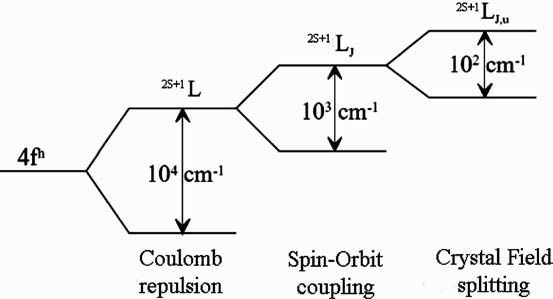
\includegraphics[height=4cm]{pics/aufspaltung.jpg}
      \caption*{\tiny Energieaufspaltung wegen Wechselwirkungen}
 \end{figure}
  \column{0.4\textwidth}
  
 \begin{figure}[!h]
\centering
      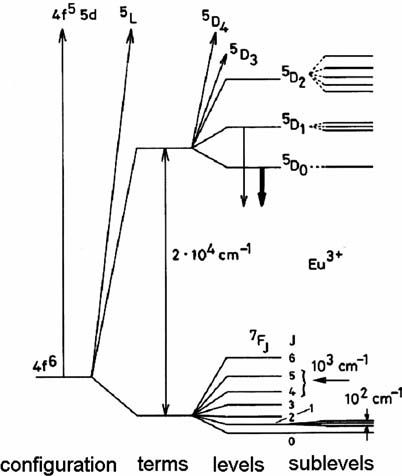
\includegraphics[height=5cm]{pics/levels.jpg}
     
      \caption*{\tiny Energieaufspaltung von \ce{Eu^{3+}}}
 \end{figure}
      \end{columns}


\end{frame}


\begin{frame}[t]\frametitle{Interkombinationsverbot}
    %jeder Übergang, bei dem sich der sich Gesamtspin geändert, ist verboten 
\begin{figure}[!h]
\centering
\begin{tikzpicture}[scale=0.8]

\drawLevel[elec = updown, pos = {(0,3)},    width = 1]{ndf1};
\drawLevel[elec = up, pos = {(1.2,3)},  width = 1]{ndf2};
\drawLevel[elec = up, pos = {(2.4,3)},  width = 1]{ndf3};
\drawLevel[elec = up, pos = {(3.6,3)},  width = 1]{ndf4};
\drawLevel[elec = up, pos = {(4.8,3)},  width = 1]{ndf5};
\drawLevel[elec = up, pos = {(6,3)},  width = 1]{ndf6};
\drawLevel[elec = none, pos = {(7.2,3)},  width = 1]{ndf7};
\node[right] at (right ndf7) {\Large \ce{^{6}_{}S _0 Gd^{3+}  } } ;


\drawLevel[elec = up, pos = {(0,1)},    width = 1]{ndf21};
\drawLevel[elec = up, pos = {(1.2,1)},  width = 1]{ndf2};
\drawLevel[elec = up, pos = {(2.4,1)},  width = 1]{ndf3};
\drawLevel[elec = up,pos = {(3.6,1)},  width = 1]{ndf4};
\drawLevel[elec = up,pos = {(4.8,1)},  width = 1]{ndf5};
\drawLevel[elec = up,pos = {(6,1)},  width = 1]{ndf6};
\drawLevel[elec = up,pos = {(7.2,1)},  width = 1]{ndf9};
\node[right] at (right ndf9) {\Large \ce{^{8}_{}S_{7/2} Gd^{3+}  } } ;
\node at (0.5,4) {$-3$};
\node at (1.5,4) {$-2$};
\node at (2.7,4) {$-1$};
\node at (4,4) {$0$};
\node at (5.5,4) {$1$};
\node at (6.5,4) {$2$};
\node at (7.5,4) {$3$};
\draw [<-, ultra thick] (left ndf1) edge[bend right]  (left ndf21);
\end{tikzpicture}
\caption{Interkombinationsverbot}

\end{figure}
\begin{itemize}
  \item Verboten, weil zu Spinpaarungen führt.
  \item die farblosen Beispiele aus den ÜM: \ce{Fe^{3+}}, \ce{Mn^{2+}}
  \item farblos auch \ce{La^{3+} f^0}, \ce{Gd^{3+} f^7},\ce{Lu^{3+} f^{14}}   
\end{itemize}
\end{frame}
\begin{frame}[t]\frametitle{Regel von Laporte}
\begin{itemize}
  \item Übergänge zwischen unterschiedlicher Parität erlaubt
  \item s- und d-Orbitale sind gerade
  \item p- und f-Orbitale sind ungerade  
\end{itemize}
   \begin{table}
      
      \begin{tabular}{cc}
\toprule
Erlaubt  & Verboten\\
\midrule
\ce{s <-> p} & \ce{d <-> d} \\
\ce{f <-> d} & \ce{f <-> f} \\
\bottomrule
\end{tabular}
\caption*{\footnotesize elektronische Übergangsarten der Lanthanoide}
    \end{table}
  

\end{frame}


\begin{frame}[t]\frametitle{Konzentration Abhängigkeit }
\begin{itemize}  
\item  \footnotesize Zur Herstellung eines Leuschtstoffs werden farblose, 
salzartige Wirststrukturen gezielt mit Metallionen dotiert (<5 mol-\%)
\item \footnotesize  Störung des Grundgitters
\begin{itemize}
 \item \footnotesize dotiertes \ce{La_2O_3:Eu} charakterisiert
  \item \footnotesize durch die Zusammensetzung \ce{La_{2-x}Eu_x O_3} (x<0.1)
\end{itemize} 
    \item \footnotesize Intensität, Polarisation und Lebensdauer hängen von Konzentration ab
  \item \footnotesize durch die Änderung der Konzentration wird Abklingszeit eingestellt 
\end{itemize}
\end{frame}



\begin{frame}[t]\frametitle{Scheelit \ce{CaWO4} als Wirtgitter}
     \begin{columns}
      \column{.5\textwidth}
              \begin{figure}[!h]
\centering
      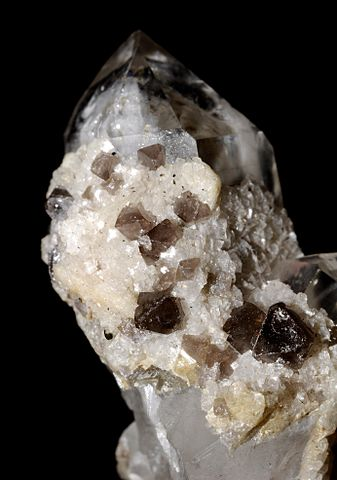
\includegraphics{pics/scheelitesurquarz.jpg}
      \caption*{\footnotesize Scheelit ist ein häufig vorkommendes Mineral}
 \end{figure}
  \column{.5\textwidth}
  
 \begin{figure}[!h]
\centering
      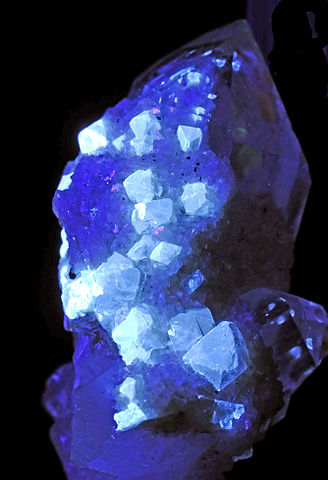
\includegraphics{pics/scheelitesurquarz2.jpg}
     
      \caption*{\footnotesize \ce{CaWO_4} unter UV-Licht}
 \end{figure}
      \end{columns}

 \begin{itemize}
      \item \footnotesize ein geringer Zusatz an Samarium verändert die Farbe ins gelborange.
    \end{itemize}   

\end{frame}


\begin{frame}[t]\frametitle{\ce{Eu,Tb}-Emission im Scheelit-Gitter}
 \begin{columns}
    \column{.6\textwidth}
    \begin{itemize}
      \item \footnotesize \ce{Eu^{3+}} erst bei Konzentration 2.5 \% \si{\mol} rot
      \item  \footnotesize empfindlicher Dipolübergang  \ce{5D_1 -> 7F_2}
    \end{itemize}
     \column{.4\textwidth}
      \begin{figure}[!h]
\centering
     \begin{tikzpicture}
\node[inner sep=0pt] (russell) at (0,0)
    {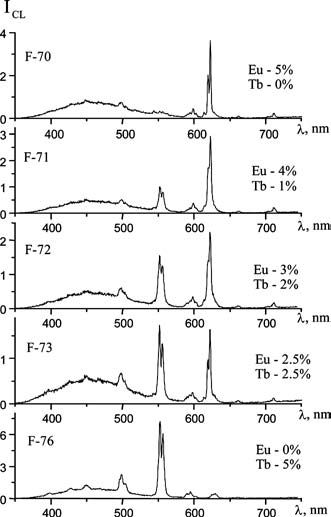
\includegraphics[scale=0.35]{pics/scheelite.jpg}};
     \colorlet{color min hsb}[hsb]{red}
  \colorlet{color max hsb}[hsb]{violet}
   \foreach \pos in {100,...,0}{
    \colorlet{my color hsb}[rgb]{color min hsb!\pos!color max hsb}
    \fill[fill=my color hsb,draw=none] (-1.7+\pos/36,-3.4) rectangle +(5mm,1mm);
  }
\end{tikzpicture}

      \caption*{\tiny \ce{CaWO4:Eu^{3+}, Tb^{3+} }}
 \end{figure}
 \end{columns}

\end{frame}

\begin{frame}[t]\frametitle{Farbeigenschaften der Lanthanoide}
     \begin{table}
      \centering
\resizebox{\linewidth}{!}{%
\begin{tabular}{cccccccccccccccc}
\toprule
 $[Xe]$ &\ce{La^{3+}} & \ce{Ce^{3+}} &\cellcolor[RGB]{ 110,194,47} \ce{Pr^{3+}} &\cellcolor[RGB]{202,99 ,138} \ce{Nd^{3+}} & \cellcolor[RGB]{ 240,42 ,242} \ce{Pm^{3+}}&\cellcolor[RGB]{  252, 255, 110} \ce{Sm^{3+}} &  \ce{Eu^{3+}} & \ce{Gd^{3+}} & \ce{Tb^{3+}}& \cellcolor[RGB]{ 163, 255, 0} \ce{Dy^{3+}} &  \cellcolor[RGB]{  255,255, 0} \ce{Ho^{3+}} & \cellcolor[RGB]{  194,171, 187}\ce{Er^{3+}} & \cellcolor[RGB]{171,228,149} \ce{Tm^{3+}} & \ce{Yb^{3+}} & \ce{Lu^{3+}}\\
   & \cellcolor[RGB]{254,225,2} \ce{Ce^{4+}} & \cellcolor{yellow}\ce{Pr^{4+}} &\cellcolor[RGB]{ 111, 0,255} \ce{Nd^{4+}} &&  &  & \cellcolor[RGB]{151,26,14} \ce{Sm^{2+}} & \ce{Eu^{2+}} & \cellcolor[RGB]{ 251, 241, 35}\ce{Dy^{4+}}&  &  & &  &\cellcolor[RGB]{ 163,79,128}\ce{Tm^{2+}}&  \cellcolor[RGB]{181,201,19}\ce{Yb^{2+}}\\
   &  & &  &  &  &  &  &  & \cellcolor[RGB]{60,0,0} \ce{Tb^{4+}} &  &  &  &  & & \\
\midrule
  4f & 0 &1 & 2 & 3 & 4 & 5 & 6 & 7 & 8 & 9 & 10 & 11 & 12 & 13& 14\\
  \bottomrule
\end{tabular}
} 
\end{table}
 
    \begin{itemize}
      \item \footnotesize Einsatz als Pigment
    \end{itemize}
\begin{figure}[!h]
\centering
      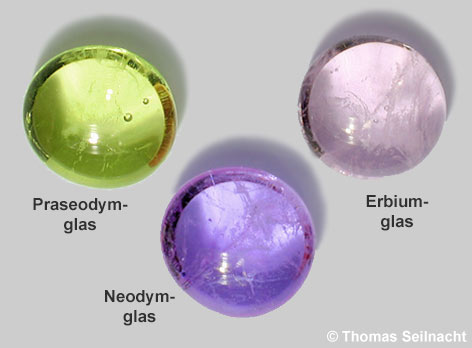
\includegraphics[scale=0.3]{pics/lantglas.jpg}
      \caption*{\footnotesize Glasperlen mit Oxiden der Lanthaniden}
 \end{figure}
\end{frame}



\begin{frame}[t]\frametitle{Lanthanoide in der Display-Technologie }
    
    \begin{tabular}{lccccc}
\toprule
\multirow{2}{*}{Leuchtstoff}& Abk. &  \ce{$\lambda$} & Abs. bei  & QE & LE  \\
& &\si{\nano\meter}&254 \si{\nano\meter}  & \% & \si{\lumen\per\watt}\\
\midrule
 \ce{BaMgAl_{10}O_{17}:Eu}& BAM & \cellcolor[wave]{450} 450  & 90 &  90 &90\\
\ce{(Ce,Tb)MgAl_{11}O_{19}}   & CAT   &  \cellcolor[wave]{542} 542  &  95 & 90& 495\\
\ce{Y_2O_3:Eu}    & YOX   &  \cellcolor[wave]{611} 611  &  75 & 90 &280\\
 \ce{BaMgAl_{10}O_{17}:Eu}  & BAM-Mn  & \cellcolor[wave]{520} 520 &  & & \\
\ce{MgGePO_{5.5}F:Mn}  & MGM  & \cellcolor[wave]{655} 655 & 95 &80 & 80\\
\ce{Sr_2P_2O_7:Eu}  & SPE  & \cellcolor[wave]{420} 420 &  & & \\
\bottomrule
\end{tabular}

\begin{figure}[!h]
\centering
      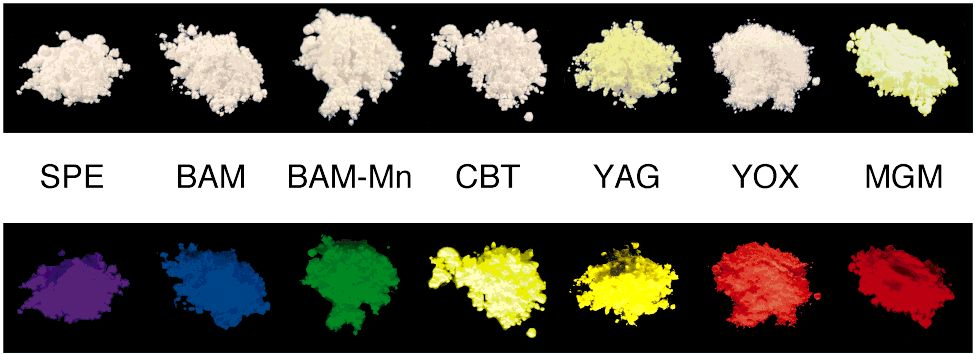
\includegraphics[scale=0.17]{pics/palette.jpg}
      \caption*{\footnotesize Handelsübliche Display-Leuchtstoffe}
 \end{figure}
\end{frame}


\begin{frame}[t]\frametitle{\small Leuchtstoffe in Lampen}
  \begin{itemize}
    \item Das Drei-Banden-Konzept
          \begin{itemize}
            \item \footnotesize Fluoreszenzlampen mit sehr guter Farbwiedergabe und hoher Lichtausbeute
          \end{itemize}
  \end{itemize}

\begin{figure}[!h]
\centering
      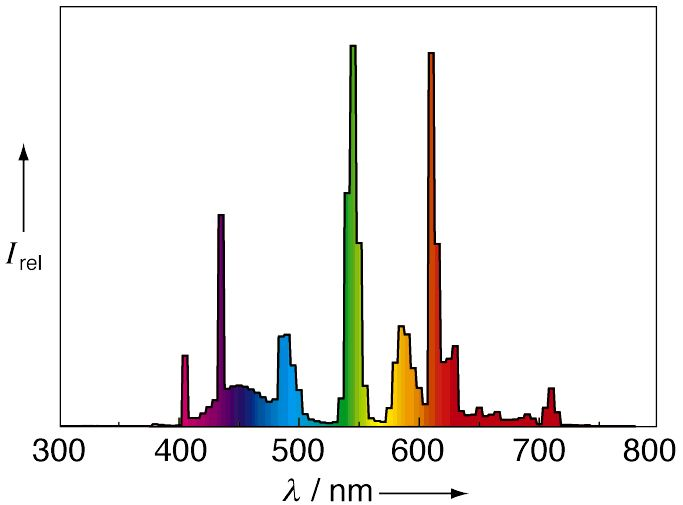
\includegraphics[scale=0.2]{pics/dd.jpg}
      \caption*{\footnotesize \ce{Emission einer Drei-Banden-Leuchtstofflampe} }
 \end{figure}


\end{frame}


\begin{frame}[t]\frametitle{Umweltfreundliche Leuchtstoffe }
  \begin{itemize}
    \item Nachtfalter reagieren auf UV-Licht
  \end{itemize}
  
\begin{figure}[!h]
\centering
      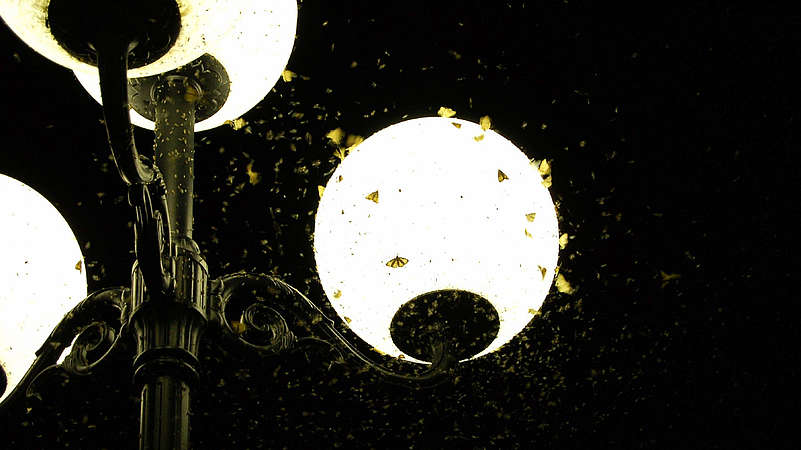
\includegraphics[scale=0.3]{pics/schwarm.jpg}
      \caption*{\footnotesize Nachtfalter um Quecksilberdampflampen }
 \end{figure}


\end{frame}





\begin{frame}[t]\frametitle{Literaturverzeichnis}
    

\begin{thebibliography}{9}
\bibitem{holeman}
E. Wiberg, \emph{Lehrbuch der Anorganische Chemie}, 102. Aufl., De Gruyter, Berlin \textbf{2007}, S. 1370.
\bibitem{nazarov}
M. Nazarov, \emph{New Generation of Eu and Tb activated phosphors}, 1., CRC, New York \textbf{2012}.
\bibitem{hoppe}
H. Höppe, \textit{Angewandte Chemie} \textbf{2009}, \textit{121}, 3626–3636.
\bibitem{ronda}
 T. Jüstel, H. Nikol, C. Ronda, \textit{Angewandte Chemie} \textbf{1998}, \textit{110}, 3250–3271.
\bibitem{yagce}
\emph{Yag-Ce}
 \url{http://www.scientificmaterials.com/products/ce-yag.php}.
\bibitem{wikilila}
\emph{Violett}
 \url{https://de.wikipedia.org/wiki/Violett}.
 \bibitem{wikilila}
\emph{Farbtemperatur}
\url{http://www.puchner.org/Fotografie/technik/physik/licht.htm}
\bibitem{wikilila}
\emph{Nachtfalter}
\url{http://www.weltderwunder.de/artikel/warum-lieben-motten-nachts-das-licht-sind-tagsueber-aber-kaum-zu-sehen/}
\end{thebibliography}
  
\end{frame}


%http://www.rsc.org/chemistryworld/News/2009/September/01090901.asp
%https://www.osapublishing.org/oe/fulltext.cfm?uri=oe-19-S3-A331
\end{document}

% Reference